\documentclass[a4paper]{article}
\usepackage[margin=1in]{geometry}%设置边距,符合Word设定
\usepackage{amssymb,amsfonts,amsmath,amsthm}
\usepackage{ctex}
\usepackage{setspace}
\usepackage{lipsum}
\usepackage{graphicx}%插入图片
\usepackage{listings}
\graphicspath{{Figures/}}%文章所用图片在当前目录下的 Figures目录

\usepackage{hyperref} % 对目录生成链接,注:该宏包可能与其他宏包冲突,故放在所有引用的宏包之后
\hypersetup{colorlinks = true,  % 将链接文字带颜色
	bookmarksopen = true, % 展开书签
	bookmarksnumbered = true, % 书签带章节编号
	pdftitle = 例一、例二论文, % 标题
	pdfauthor =刘正浩} % 作者
\bibliographystyle{plain}% 参考文献引用格式
\newcommand{\upcite}[1]{\textsuperscript{\cite{#1}}}

\renewcommand{\contentsname}{\centerline{Contents}} %经过设置word格式后,将目录标题居中

\lstset{
	basicstyle = \small
}

\title{\heiti\zihao{2} 例一、例二论文}
\author{\songti 刘正浩}
\date{\today}


\begin{document}
	\maketitle
	\thispagestyle{empty}

% \begin{abstract}
% 	\lipsum[2]
% \end{abstract}

\tableofcontents

	\section{例一}
		\begin{figure}[htbp]
			\centering
			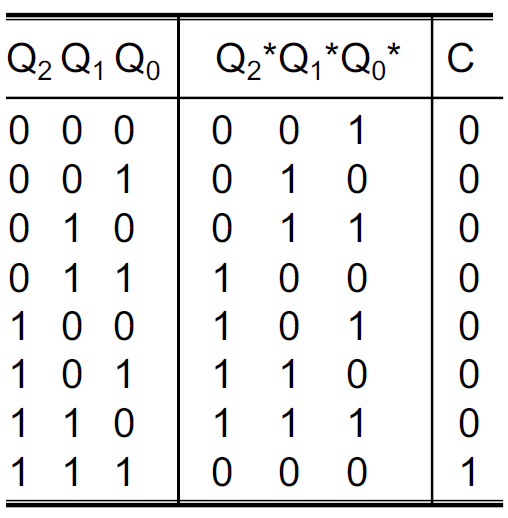
\includegraphics[scale=0.3]{例一转移输出表.png}
			\caption{例一 转移/输出表}
		\end{figure}
		在得到如图的状态转移表之后,可以通过卡诺图求得状态转移方程和输出方程。三个状态转移方程和一个输出方程如下:
		\begin{align}
			Q_0^* &= Q_0'\\  
			Q_1^* &= Q_1' Q_0 + Q_1 Q_0'\\  
			Q_2^* &= Q_2' Q_1 Q_0 + Q_2 Q_1' + Q_2 Q_0'\\
			C &= Q_2 Q_1 Q_0
		\end{align}
		如果使用D触发器搭建状态机,则激励方程为
		\begin{align}
			D_0 &= Q_0'\\  
			D_1 &= Q_1' Q_0 + Q_1 Q_0'\\  
			D_2 &= Q_2' Q_1 Q_0 + Q_2 Q_1' + Q_2 Q_0'
		\end{align}
		由于使用结构化描述方式进行设计,则在代码中组合逻辑部分如下:
		\begin{lstlisting}
			--第一个触发器之前的组合逻辑--------------
			d_0 <= not q_0;
			--第二个触发器之前的组合逻辑--------------
			d_1 <= ((not q_1) and (q_0)) or ((q_1) and (not q_0));
			--第三个触发器之前的组合逻辑--------------
			d_2 <= ((not q_2)and(q_1)and(q_0)) or
			       ((q_2)and(not q_1)) or
			       ((q_2)and(not q_0));
			
			c <=  q_0 and q_1 and q_2;
		\end{lstlisting}
		设计完成后,对状态机进行仿真。仿真结果如下图:
		\begin{figure}[htbp]
			\centering
			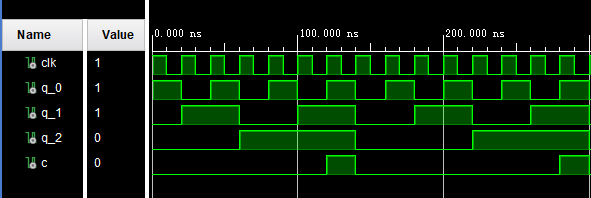
\includegraphics[scale=1]{例一仿真结果.png}
			\caption{例一仿真结果}
		\end{figure}
	
	\section{例二}
		\begin{figure}[htbp]
			\centering
			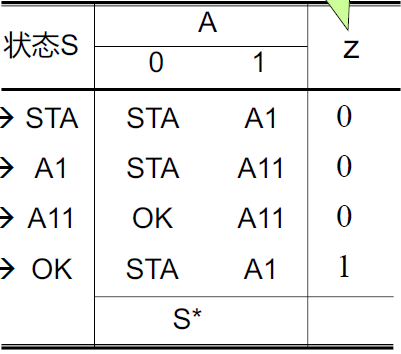
\includegraphics[scale=0.8]{例二状态转换表.png}
			\caption{例二状态转换表}
		\end{figure}
		用A表示串行输入的数据,用Z表示检测结果,可以得到Moore机的状态转换表.
		有了状态转换表,可以很容易写出三段式状态机中的状态转移部分。
		\begin{lstlisting}
			STATE_TRANS :process(current_state, a)  --状态转换
            begin
                case current_state is
                    when sta =>
                        if(a = '1')then
                            next_state <= a1;
                        else
                            next_state <= current_state;
                        end if;
                    when a1 =>
                        if(a = '1')then
                            next_state <= a11;
                        else
                            next_state <= sta;
                        end if;
                    when a11 =>
                        if(a = '1')then
                            next_state <= current_state;
                        else
                            next_state <= ok;
                        end if;
                    when ok =>
                        if(a = '1')then
                            next_state <= a1;
                        else
                            next_state <= sta;
                        end if;
                    when others =>
                        next_state <= current_state;
                end case;
            end process;
		\end{lstlisting}
		其余代码详见项目代码。\par
		仿真的结果如下图。(测试序列为01110010110)
		\begin{figure}[htbp]
			\centering
			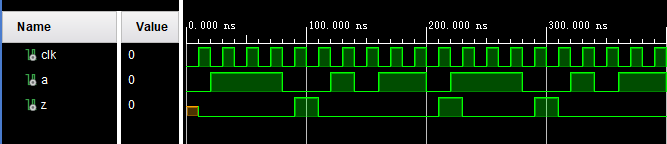
\includegraphics[scale=0.85]{例二仿真结果.png}
			\caption{例二仿真结果}
		\end{figure}
\end{document}